\subsection{Buffer lineal}


\begin{enumerate}
    \item 

Para lograr una linea de retardo se implementa un buffer lineal en lenguaje C, integrado a MATLAB mediante el uso de \textit{s-function}.

El siguiente código muestra la función en lenguaje C que implementa el buffer.

    \begin{lstlisting}
    
#define N (32000)
double retardo_lineal(double input) {
	// Buffer lineal
	static double buffer[N];
    
    //Inicializacion del buffer
	static int flag = 1;
    
	if (flag == 1) {
		for (int i = 0; i < N; i++) {
			buffer[i] = 0;
		}
		flag = 0;
	}

	double output = buffer[N - 1];

	for (int idx = N - 1 ; idx >= 1; idx--) {
		buffer[idx] = buffer[idx -1];
	}
	buffer[0] = input;
	return output;
}

    \end{lstlisting}
    
    Donde la entrada a la función es una muestra actual n de la señal que se desea retardar, dato que se guarda en el buffer de N elementos, mientras que la salida retornada por la función corresponde a la primera posición del buffer, es decir el dato guardado  n - N.
    
    
    
    
    Para verificar el correcto funcionamiento de este retardo lineal implementado se escoge el archivo de audio \textit{sonidos\_de\_voz\_16\_8.wav} ya que por la manera en la que está distribuida la información  en el tiempo en este archivo (viendo la forma de onda a graficar los datos del arhcivo) un retardo en un mensaje hablado es significativamente notorio. En este punto es necesario comentar la relación que existe entre el \textbf{tiempo de retardo}  y la frecuencia de muestreo \textbf{Fs} asociado a las señales a trabajar, el inverso de esta frecuencia corresponde al periodo de muestreo , que al ser multiplicado por la cantidad de muestras que se desean almacenar en el buffer se obtiene el tiempo total de retardo provocado en la señal. 
    
    
    La frecuencia de muestreo de la señal escogida es de  $8~kHz$, por lo que con un N de 32000 muestras se debiera obtener un retardo de $4~s$ como se muestra a continuación
    
    $$T_{retardo} = \frac{1}{Fs}\cdot N = \frac{1}{8 ~kHz}\cdot 32000 = 4~s$$
    
     Se crean los bloques necesarios para hacer uso de la \textit{s-Function} creada, importar el archivo de audio y un scope para poder observar y comparar las señales obteniendo de esta forma las gráficas presentes en la figura \ref{retardo_lineal}  
    
    Cabe destacar que si bien la guía propone un retardo de $N = 100$ , debido a la frecuencia de muestreo que posee el archivo de audio esta cifra provocaría un retardo despreciable por lo que se optó por un  valor de $N = 32000$, tal como se mencionó antes.
    
    \begin{figure}[H]
        \centering
        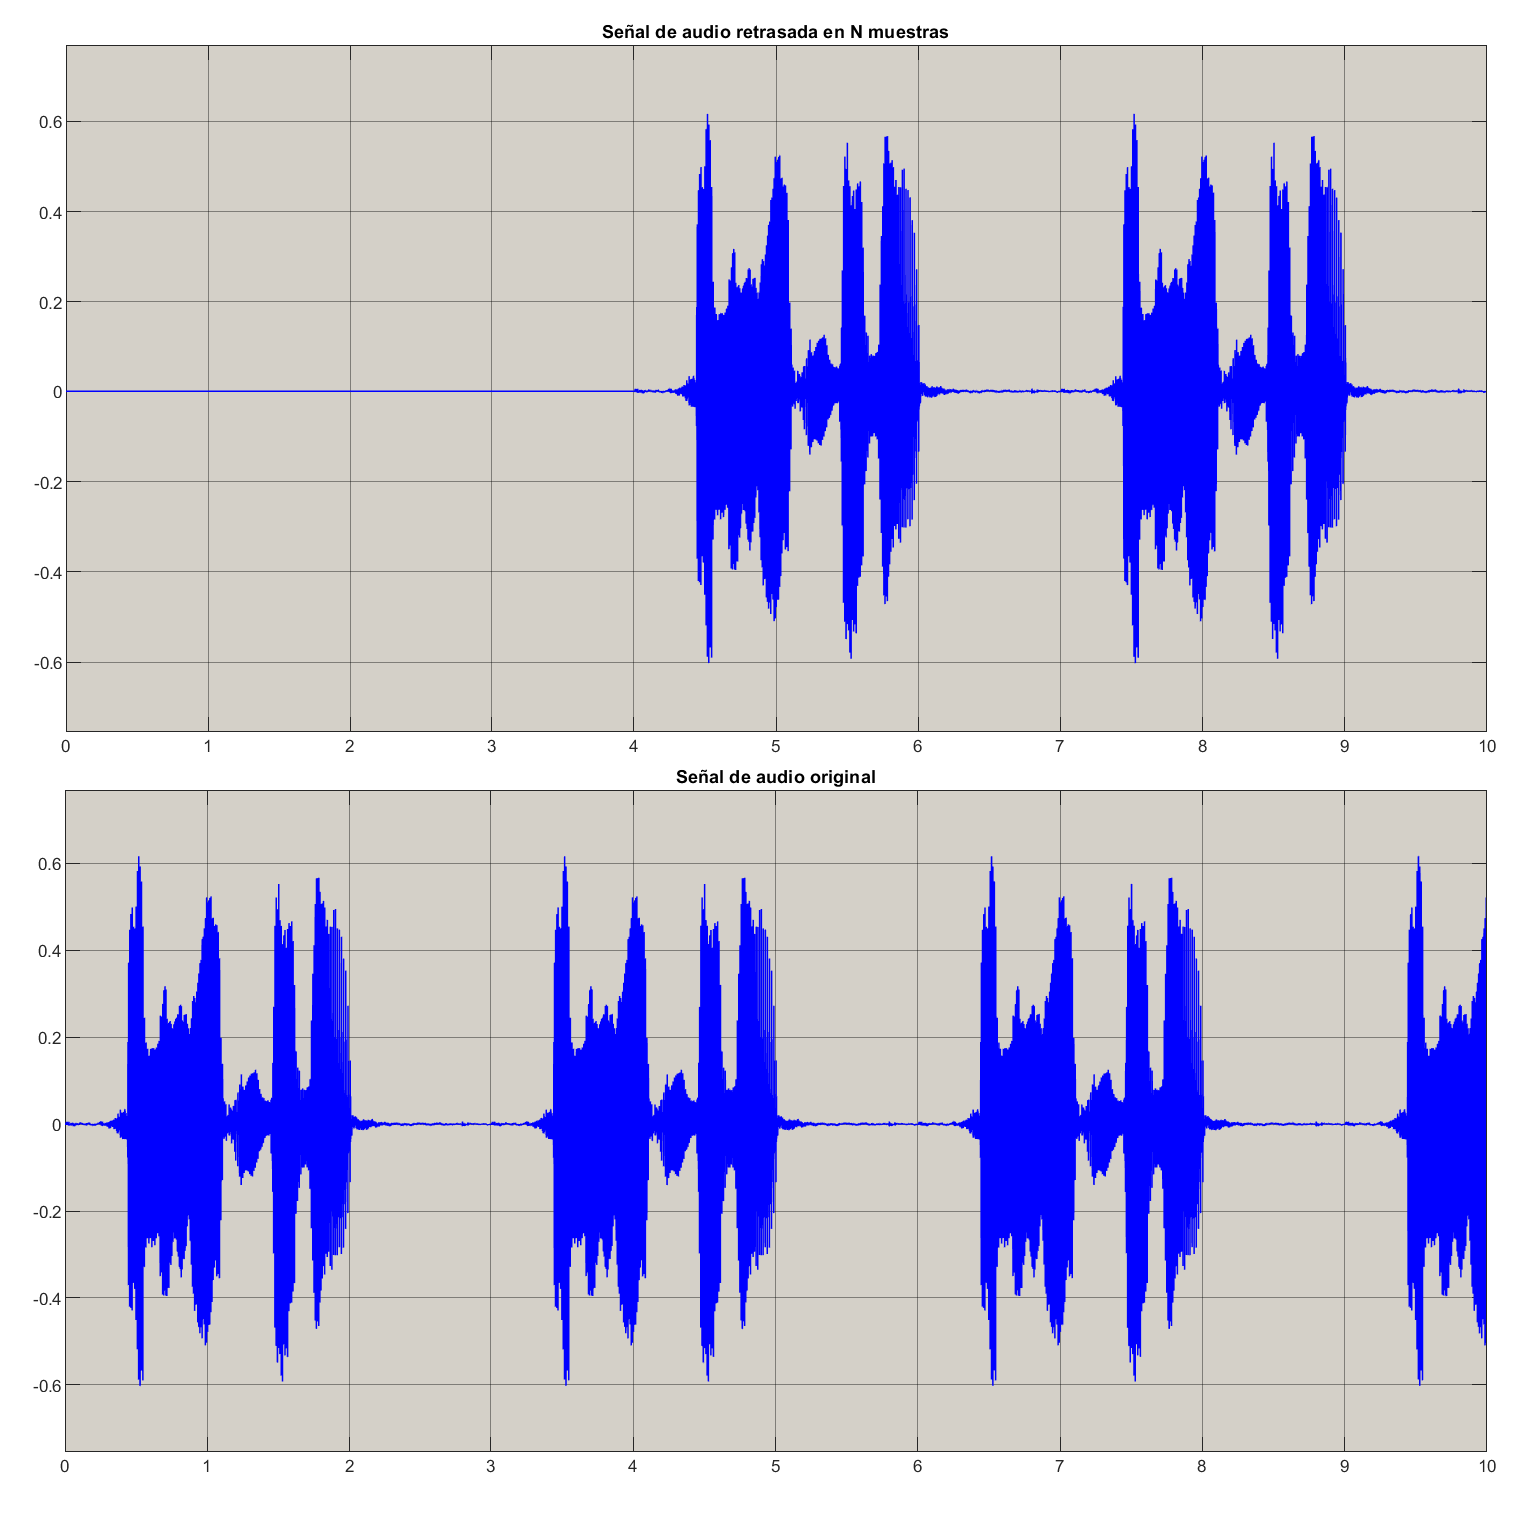
\includegraphics[scale = 0.5]{Figuras/p31_retardo_lineal.eps}
        \caption{Gráfica del resultado de aplicar el retardo lineal implementado a una señal de audio.}
        \label{retardo_lineal}
    \end{figure}
    
    En la figura anterior se puede ver que tal como se esperaba el buffer lineal implementado provoca un retardo de $4~s$ respecto de la señal de audio original desplazándola en 32000 muestras  hacia la derecha.
    
    \item
    
    De la misma manera que en el apartado anterior, se implementa una linea de retardo usando código en lenguaje C pero esta vez haciendo uso de un \textbf{buffer circular} en tiempo real, el código de implementación es el siguiente
    
    \newpage
    \begin{lstlisting}
    
    #define n (32000)
    double retardo_circular(double input) {
    
    
    
    static double buffer[n]; //Crea buffer tamaño n
    	
    //inicialica el "puntero" idx en la ultima posicion
    static  int idx = n-1;  
    
    //Bloque para inicializar el buffer con ceros
    static int flag = 1;
    
    if (flag == 1) 
    {
    	for (int i = 0; i < n; i++) 
    	{
    		buffer[i] = 0;
    	}
        flag = 0;
    } 
    //Fin inicializacion del Buffer
    
    double output = buffer[idx]; //Lee dato del Buffer
    buffer[idx] = input;  //Actualiza el dato en posicion idx
    idx = ((idx+1)%n); //Actualiza posicion idx
    
    
    return (output);
    }

    \end{lstlisting} 
    
    Al graficar la señal original y la que sufrió el retardo debido usando buffer circular son practicamente idénticas  a las gráficas obtenidas con el buffer de tipo lineal ya que ambas implementaciones cumplen el objetivo que es provocar un retardo.
    
\item Para comparar la eficiencia de ambos métodos para retardo implementados,  usando el modo \textit{PROFILE} de simulink se estudian los tiempos de ejecución de la simulación que requieren ambas \textit{s-Function} (la asociada a buffer llineal y a buffer circular respectivamente). De este modo se obtuvieron los datos que se presentan en los cuadros \ref{lin_tabl} y \ref{circ_tabl}




\begin{table}[H]
        \centering
        \begin{tabular}{|c|c|c|c|c|c|c|}
        \hline
 N  & Scope & From multimedia file & s-Function & Simulacion & Total \\
 \hline
 20 &0,042	&0,091	&0,019	&0,563	&0,612 \\
 \hline
 200 & 0,044 &	0,091	&0,024&	0,488&	0,647 \\
 \hline
 2000 &0,045 &	0,099	&0,079&	0,482&	0,705\\
 \hline

 20000 & 0,055&	0,113	&0,617	&0,433&	1,2185\\
 \hline
 
        \end{tabular}
        \caption{Tiempos de ejecución en segundos de la simulación haciendo uso de  buffer lineal.}
        \label{lin_tabl}
    \end{table}





 \begin{table}[H]
        \centering
        \begin{tabular}{|c|c|c|c|c|c|c|}
        \hline
         N  & Scope & From multimedia file & s-Function & Simulacion & Total \\
         \hline
         20 & 0,120	 &0,0860&	0,0170	&0,175&	0,398 \\
         \hline
         200 & 0,107 &	0,0860	&0,0170&	0,478	&0,688 \\
         \hline
         2000 & 0,126	&0,0880&	0,0180&	0,475&	0,707 \\
         \hline
        
         20000 & 0,100 &	0,0800	&0,0170&	0,178	&0,375\\
         \hline

        \end{tabular}
        \caption{Tiempos de ejecución en segundos de la simulación haciendo uso de  buffer circular.}
        \label{circ_tabl}
    \end{table}





De las tablas resumen anteriores se puede ver  cómo varía la eficiencia en ejecución de los buffers lineal y circular implementados dependiendo del valor de N correspondiente al número de  muestras que se deben almacenar en el buffer.


Cuando N tiene un valor de 20 muestras  ambos buffers tienen un rendimiento similar cercano a los $20~ms$. 

Al pasar N por los valores siguientes de 200, 2000 y 20000 el tiempo que requiere la simulación para ejecutar el bloque del buffer circular se mantiene relativamente constante   en el mismo valor anterior cercano a los  $20~ms$, mientras que el buffer lineal aumenta el tiempo requerido en una proporción similar al incremento en el valor de N haciendo notar que para implementaciones que requieran pocas muestras se pueden utilizar ambos tipos de buffer, lineal y circular indistintamente, pero que si el contexto requiere almacenar grandes cantidades de datos en el buffer, el de tipo circular es claramente superior al momento de cumplir con esa labor. Esto se debe a que en esencia el buffer lineal requiere mover todos los datos dentro de las posiciones del arreglo en el que esta implementado, recorriendo dicho arreglo mediante un ciclo iterativo  (\texttt {for}, por ejemplo), por lo que si este buffer tiene un tamaño considerable el ciclo iterativo encargado de recorrerlo para mover los datos de las posiciones tendría que realizar más iteraciones para mover todos los datos provocando un evidente desmedro en la eficiencia de este tipo de buffer. 


\item Al cambiar el tipo de variable con las que trabaja la linea de retardo basada en buffer lineal de tipo \texttt{double} a \texttt{int16}, considerando un valor N de 20000 muestras y medir el tiempo de ejecución con el modo PROFILE de simulink, se obtuvo un tiempo para la \textit{s-Function} de \textbf{0.635~ms}, mayor al obtenido con el mismo buffer, mismo valor de N   y tipo de datos \texttt{double} que fue de \textbf{0.617~ms} (ver cuadro 1). Si bien la diferencia no es significativa  correspondiendo ambas cifras al mismo es importante notar que efectivamente existe y se debe a que se está trabajando con una arquitectura diseñada y optimizada para trabajar con datos de 64 bits,  al forzar a que el procesador trabaje con otro tipo de datos, este debe implementar nuevas instrucciones que realicen la conversión de datos desde el tipo de dato por defecto al indicado, en este caso \texttt{int16}.

Se concluye entonces que el tiempo de ejecución efectivamente depende de la arquitectura que se esté usando, siendo óptimo el intentar trabajar con tipos de datos que coincidan con el numero de bits para los que fue diseñado el dispositivo que vaya a procesarlos, por ejemplo un \textit{arduino UNO} presentaría mayor eficiencia usando datos de 8 bits  así como una tarjeta  \textit{MSP430} optimizaría sus funciones trabajando con datos de 16 bits pues no tendrían que agregar instrucciones dedicadas a la conversión de datos.


\item Utilizando el modelo Simulink bypass del material del laboratorio se aprovecha el retardo de procesamiento de la señal del micrófono al pasar por Simulink y retornar a los  audífonos. Con esta simulación se analiza como afecta este retardo a la capacidad de habla.

Al desarrollar este ejercicio, intentando leer o hablar fluidamente, esta simple acción se complica bastante al escuchar la señal de voz retardada a través de los audífonos,  esto se puede deber a que si se hace la analogía con un sistema de control en lazo cerrado, la señal de salida que se mide por los audífonos que posee retardo,  al acoplarse con la señal de entrada (voz hablada) la suma de estas señales provoca un error significativo a la entrada del controlador (en este caso el cerebro), impidiendo elaborar acciones  acertadas,  que en el contexto sería continuar la lectura o el habla normal.



\end{enumerate}
